\documentclass{article}
\usepackage{graphicx,fancyhdr,amsmath,amssymb,amsthm,subfig,url,hyperref}
\usepackage[margin=1in]{geometry}
\usepackage{enumerate}
\usepackage{algorithm}
\usepackage{algpseudocode}
\usepackage{pifont}
 \usepackage{color}


\usepackage{tikz}
\usepackage{tabularx}
\usetikzlibrary{shapes.geometric}
\usetikzlibrary{arrows}

\renewcommand{\algorithmicrequire}{\textbf{input:}}

%----------------------- Macros and Definitions --------------------------

%%% FILL THIS OUT
\newcommand{\studentname}{Nico Chaves, Mike Schoenhals, Junjie (Jason) Zhu}
\newcommand{\suid}{jjzhu}
\newcommand{\exerciseset}{}
%%% END
\renewcommand{\theenumi}{\bf \Alph{enumi}}

%\theoremstyle{plain}
%\newtheorem{theorem}{Theorem}
%\newtheorem{lemma}[theorem]{Lemma}

\fancypagestyle{plain}{}
\pagestyle{fancy}
\fancyhf{}
\fancyhead[RO,LE]{\sffamily\bfseries\large  CME 307 Final Project, Stanford University}
\fancyhead[LO,RE]{\sffamily\bfseries\large ADMM Techniques}
% \fancyfoot[LO,RE]{\sffamily\bfseries\large \studentname: \suid @stanford.edu}
\fancyfoot[RO,LE]{\sffamily\bfseries\thepage}
\renewcommand{\headrulewidth}{1pt}
\renewcommand{\footrulewidth}{1pt}

\graphicspath{{figures/}}

%-------------------------------- Title ----------------------------------

\title{ADMM Techniques for Linear \& Semidefinite Programming }
\author{\studentname}

%--------------------------------- Text ----------------------------------

\begin{document}
\maketitle

%%%%%%
\section{Introduction}
The alternating direction method of multipliers (ADMM) is a 1st order optimization method. In this project, we experimented with variants of ADMM applied to the following optimization problems. \\
Linear Programming Primal:
\begin{align}
\min_{\mathbf{x}} &\quad \mathbf{c}^T\mathbf{x} \tag{LP}\label{eq:LP} \\
\text{subject to } &\quad  A \mathbf{x} = \mathbf{b},  \nonumber \\
&\quad \mathbf{x} \geq \mathbf{0} \nonumber 
\end{align}
Linear Programming Dual:
\begin{align}
\max_{\mathbf{y}, \mathbf{s}} &\quad \mathbf{b}^T\mathbf{y}  \tag{LD}\label{eq:LD} \\
\text{subject to } &\quad  A^T \mathbf{y}  + \mathbf{s} = \mathbf{c},  \nonumber \\
&\quad \mathbf{s} \geq \mathbf{0} \nonumber.
\end{align}
SDP Primal:
\begin{align}
\min_{X} &\quad C\bullet X  \tag{SDP}\label{eq:SDP} \\
\text{s.t.} &\quad \mathcal{A}X=\mathbf{b} \nonumber \\
&\quad X\succeq \mathbf{0} \nonumber
\end{align}
SDP Dual:
\begin{align}
\max_{\mathbf{y},S} &\quad \mathbf{b}^{T}\mathbf{y} \tag{SDD}\label{eq:SDD}  \\
\text{s.t.} &\quad \mathcal{A}^{T}\mathbf{y}+S=C \nonumber \\
&\quad S\succeq\mathbf{0} \nonumber
\end{align}

For \eqref{eq:LP} and \eqref{eq:LD}, we also experimented with block splitting, interior point methods, and preconditioning. Our solvers and experiments are available online: https://github.com/nmchaves/admm-for-lp. 

%%%%%%%%%%
\section{Basic ADMM for Linear Programming}
In this section, we describe the ADMM update procedures for solving \eqref{eq:LP} and \eqref{eq:LD}.

\subsection*{Primal Update}
We re-formulate the primal LP problem as:
\begin{align}
\text{minimize}_{ \mathbf{x}_{1}, \mathbf{x}_{2}} &\quad \mathbf{c}^T\mathbf{x}_1 \tag{LPR}\label{eq:LPR} \\
\text{subject to  \ \  } &\quad  A \mathbf{x}_{1} = \mathbf{b},  \nonumber \\
&\quad \mathbf{x}_{1}  - \mathbf{x}_{2} = \mathbf{0},  \nonumber \\
&\quad \mathbf{x}_{2} \geq \mathbf{0} \nonumber 
\end{align}
and consider the augmented Lagrangian function:
\[
L^{P}(\mathbf{x}_{1},\mathbf{x}_{2},\mathbf{y} ,\mathbf{s})=\mathbf{c}^{T}\mathbf{x}_{1}-\mathbf{y}^{T}\left(A\mathbf{x}_{1}-\mathbf{b}\right)-\mathbf{s}^{T}\left(\mathbf{x}_{1}-\mathbf{x}_{2}\right)+\frac{\beta}{2}\left(\left\Vert A\mathbf{x}_{1}-\mathbf{b}\right\Vert ^{2}+\left\Vert \mathbf{x}_{1}-\mathbf{x}_{2}\right\Vert ^{2}\right)
\]
The decision variable updates are given by (see Appendix for derivation):
\begin{align}\label{eq:x1_primal_update}
\mathbf{x}_{1}^{k+1} = \left(A^{T}A+I\right)^{-1}\left(\frac{1}{\beta}A^{T}\mathbf{y}^k+\frac{1}{\beta}\mathbf{s}^k-\frac{1}{\beta}\mathbf{c}+A^{T}\mathbf{b}^k+\mathbf{x}_{2}^k\right)
\end{align}
\begin{align}
{x}_{2,j}^{k+1} = \max\left\{ {x}_{1,j}^{k+1}-\frac{1}{\beta}{s}_j^k,0\right\} \text{ for $j = 1,..,n$}.
\end{align}
\begin{align}\label{eq:y_primal_update}
\mathbf{y}^{k+1} &= \mathbf{y}^{k} + \beta (A \mathbf{x}_1^{k+1}  - \mathbf{b}) 
\end{align}
\begin{align}\label{eq:s_primal_update}
\mathbf{s}^{k+1} &= \mathbf{s}^{k}  - \beta  (\mathbf{x}_1^{k+1}  -\mathbf{x}_2^{k+1} )
\end{align}
We terminate when the solution is primal feasible, i.e., $A \mathbf{x}_1^{k+1}  - \mathbf{b} \approx \mathbf{0}$ and $\mathbf{x}_1^{k+1}  -\mathbf{x}_2^{k+1} \approx \mathbf{0}$.

%%%%%%%%%%
\subsection*{Dual Update}
We reformulate \eqref{eq:LD} as a minimization problem:
\begin{align}
\text{minimize}_{\mathbf{y}, \mathbf{s}} &\quad -\mathbf{b}^T\mathbf{y}  \tag{LDR}\label{eq:LDR} \\
\text{subject to } &\quad  A^T \mathbf{y}  + \mathbf{s} = \mathbf{c},  \nonumber \\
&\quad \mathbf{s} \geq \mathbf{0} \nonumber
\end{align}
The dual's augmented Lagrangian function is then:
\[
L^{d}(\mathbf{y},\mathbf{s},\mathbf{x})=-\mathbf{b}^{T}\mathbf{y}-\mathbf{x}^{T}\left(A^{T}\mathbf{y}+\mathbf{s}-\mathbf{c}\right)+\frac{\beta}{2}\left\Vert A^{T}\mathbf{y}+\mathbf{s}-\mathbf{c}\right\Vert ^{2}.
\]
The decision variable updates are given by (see Appendix for derivation):
\begin{align}\label{eq:y_dual_update}
\mathbf{y}^{k+1} = \left(AA^{T}\right)^{-1}\left(\frac{1}{\beta}\left(A\mathbf{x}^{k}+\mathbf{b}\right)-A\mathbf{s}^{k}+A\mathbf{c}\right),
\end{align}
\begin{align}\label{eq:s_dual_update}
s_j^{k+1} = \max\left\{ \frac{1}{\beta}{x}_j^k-(A^{T}\mathbf{y}^{k+1})_j+{c}_j,0\right\}  \text{ for $j = 1,..,n$}.
\end{align}
We update $\mathbf{x}$ using
\begin{align}\label{eq:x_dual_update}
\mathbf{x}^{k+1} = \mathbf{x}^k - \beta\left(A^T \mathbf{y}^{k+1} + \mathbf{s}^{k+1} - \mathbf{c}\right).
\end{align}
We terminate and declare optimality when $A \mathbf{x}^{k+1} + \mathbf{b} \approx \mathbf{0}$. Note: since we converted the problem to a minimization, the final $\mathbf{x}$ value will be non-positive. As a result, we must negate it to obtain the solution to the original problem.

%%%%%%%%%%%%%%%%%%%%%%%%%%%%
\section{Interior-Point ADMM for LP}

\subsection*{Interior Point Primal LP Updates}
Here we modify the formulation in \eqref{eq:LPR} using the log barrier function:
\begin{align}
\min_{ \mathbf{x}_{1}, \mathbf{x}_{2}} &\quad \mathbf{c}^T\mathbf{x}_1 - \mu \sum_j \ln( {x}_{2,j} )\tag{LPRB}\label{LPRB} \\
\text{subject to  \ \  } &\quad  A \mathbf{x}_{1} = \mathbf{b},  \nonumber \\
&\quad \mathbf{x}_{1}  - \mathbf{x}_{2} = \mathbf{0} \nonumber
\end{align}
The constraint $\mathbf{x}_{2} > \mathbf{0}$ is now implicit. The augmented Lagrangian function is given by
\[
L_{\mu}^{p}(\mathbf{x}_{1},\mathbf{x}_{2},\mathbf{y}, \mathbf{s})=\mathbf{c}^{T}\mathbf{x}_{1}-\mu\sum_{j}\ln\left(x_{2,j}\right)-\mathbf{y}^{T}\left(A\mathbf{x}_{1}-\mathbf{b}\right)-\mathbf{s}^{T}\left(\mathbf{x}_{1}-\mathbf{x}_{2}\right)+\frac{\beta}{2}\left(\left\Vert A\mathbf{x}_{1}-\mathbf{b}\right\Vert ^{2}+\left\Vert \mathbf{x}_{1}-\mathbf{x}_{2}\right\Vert ^{2}\right).
\]
The $\mathbf{x}_1$ update is the same as \eqref{eq:x1_primal_update}. The 1st order gradient condition for $\mathbf{x}_2$ is
\begin{align}
s_j - \frac{\mu}{x_{2,j}} + \beta(x_{2,j} - x_{1,j}) = 0
\end{align}
which yields the update
\begin{align}
x_{2,j} = \frac{1}{2\beta}\left(\beta x_{1,j} - s_j  + \sqrt{\beta^2 x_{1,j}^2 - 2\beta s_j x_{1,j} + s_j^2 + 4\beta\mu } \right), \text{ for $j = 1,..,n$}
\end{align}
The update equations for $\mathbf{y}$ and $\mathbf{s}$ remain the same as in \eqref{eq:y_primal_update} and \eqref{eq:s_primal_update}. At the end of each iteration, we update $\mu^{k+1} = \gamma \mu^k$ for some constant $\gamma<1$, and the termination condition remains the same as the non-interior-point method. 

\subsection*{Interior Point Dual LP Updates}
We modify \eqref{eq:LDR} using the log barrier function:
\begin{align}
\min_{\mathbf{y}, \mathbf{s}} &\quad -\mathbf{b}^T\mathbf{y} - \mu \sum_j \ln (s_j)  \tag{LDRB}\label{LDRB} \\
\text{subject to } &\quad  A^T \mathbf{y}  + \mathbf{s} = \mathbf{c}  \nonumber
\end{align}
The constraint $\mathbf{s} > \mathbf{0}$ is now implicit. The augmented Lagrangian function is given by
\[
L_{\mu}^{d}(\mathbf{y},\mathbf{s},\mathbf{x})=-\mathbf{b}^{T}\mathbf{y}-\mu\sum_{j}\ln\left(s_{j}\right)-\mathbf{x}^{T}\left(A^{T}\mathbf{y}+\mathbf{s}-\mathbf{c}\right)+\frac{\beta}{2}\left\Vert A^{T}\mathbf{y}+\mathbf{s}-\mathbf{c}\right\Vert ^{2}.
\]
The $\mathbf{y}$ update remains the same as \eqref{eq:y_dual_update}. Using the 1st order gradient condition for $\mathbf{s}$
\begin{align}
- \frac{\mu}{s_j} + x_j  + \beta \left(s_j - (\mathbf{c} - (A^T \mathbf{y}))_j\right)= 0
\end{align}
we obtain the $\mathbf{s}$ update
\begin{align}
s_j = \frac{1}{2\beta}\left(\beta (\mathbf{c} - (A^T \mathbf{y}))_j + x_j  + \sqrt{\beta^2 (\mathbf{c} - (A^T \mathbf{y}))_j^2 - 2\beta (\mathbf{c} - (A^T \mathbf{y}))_j x_{j} + x_j^2 + 4\beta\mu } \right), \text{ for $j = 1,..,n$}
\end{align}
The update equation for $\mathbf{x}$ remains the same as in \eqref{eq:x_dual_update}. As in the primal interior-point algorithm, we update $\mu^{k+1} = \gamma \mu^k$ for some constant $\gamma<1$ at the end of each iteration, and the termination condition remains the same as the non-interior-point method.

%%%%%%%%%%
\section{Multi-Block ADMM for LP}

As shown in the previous section, certain ADMM update steps require computation of a potentially large matrix inverse. This computation may become the bottleneck for sufficiently large problems. Splitting the decision variables into blocks may reduce the runtime, because one would need to compute multiple small matrix inverses instead of a single large matrix inverse.

However, when the decision variables are separable, it may not be necessary to apply block updates on them. At the end of each iteration, these separable variables would take identical values no matter how they are grouped. Thus, we only need to consider the cases where we split $\mathbf{x_1}$ in the primal problems (i.e.,  \eqref{eq:LPR} and \eqref{LPRB}) or $\mathbf{y}$ in the dual problems (i.e.,  \eqref{eq:LDR} and \eqref{LDRB}).

\subsection*{Primal ADMM with Block Splitting}

Consider splitting the problem into $B$ blocks of equal size as follows:
\[
\mathbf{x}_{1}=\begin{bmatrix}
\mathbf{x}_{1,1}\\
\mathbf{x}_{1,2}\\
\vdots \\
\mathbf{x}_{1,B}
\end{bmatrix},
 \ \  
A=\begin{bmatrix}A_{1} & A_{2} & \dots & A_{B} \end{bmatrix},
\ \ 
\mathbf{c}=\begin{bmatrix}
\mathbf{c}_{1}\\
\mathbf{c}_{2}\\
\vdots \\
\mathbf{c}_{B}
\end{bmatrix}
\]

Let $U$ denote the set of blocks which have already been updated at the current iteration. To update block $i$ of $\mathbf{x}_{1}$, we compute:
\[
\mathbf{x}_{1,i}^{k+1}=\left(A_{i}^{T}A_{i}+I\right)^{-1}\left(\frac{1}{\beta}A_{i}^{T}\mathbf{y}+\frac{1}{\beta}\mathbf{s}_{i}-\frac{1}{\beta}\mathbf{c}_{i}+A_{i}^{T}\mathbf{b}+\mathbf{x}_{2,i}^{k}-\sum_{j\neq i,j\in U}A_{i}^{T}A_{j}\mathbf{x}_{1,j}^{k+1}-\sum_{j\neq i,j\notin U}A_{i}^{T}A_{j}\mathbf{x}_{1,j}^{k}\right)
\]
where $A_{i}$ refers to the $i^{\text{th}}$ block of columns of $A$. See the Appendix for a derivation.

\subsection*{Dual ADMM with Block Splitting}

Consider splitting the problem into $B$ blocks of equal size as follows:
\[
\mathbf{y}=\begin{bmatrix}\mathbf{y}_{1}\\
\mathbf{y}_{2}\\
\vdots \\
\mathbf{y}_{B}
\end{bmatrix},
\ \
A^{T}=\begin{bmatrix}A_{1}^{T} & \dots & A_{B}^{T}\end{bmatrix},
\ \ 
\mathbf{b}=\begin{bmatrix}\mathbf{b}_{1}\\
\mathbf{b}_{2} \\
\vdots \\
\mathbf{b}_{B}
\end{bmatrix}
\]



Let $U$ denote the set of blocks which have already been updated at the current iteration. To update block $i$ of $\mathbf{y}$:
\[
\mathbf{y}_{i}^{k+1}=\left(A_{i}A_{i}^{T}\right)^{-1}\left(\frac{1}{\beta}\left(A_{i}\mathbf{x}+\mathbf{b}_{i}\right)-A_{i}\left(\mathbf{s}^{k}-\mathbf{c}\right)-\sum_{j\neq i,j\in U}A_{i}A_{j}^{T}\mathbf{y}_{j}^{k+1}-\sum_{j\neq i,j\notin U}A_{i}A_{j}^{T}\mathbf{y}_{j}^{k}\right)
\]
See the Appendix for a derivation.

%%%%%%%%%%
\section{Preconditioning}
In this report, we demonstrate that preconditioning can help ADMM solve linear programs in fewer iterations. After preconditioning the system, we solve the problem using the modified constraints: 
\begin{equation}
A' x = \mathbf{b}'
\end{equation}
where $A'$ and $\mathbf{b}'$ are the results of preconditioning $A$ and $\mathbf{b}$, respectively.
\subsection*{Standard Preconditioning}
To apply ``standard" preconditioning to a linear programming problem, one first computes 
\begin{align}
A' = (AA^T )^{-1/2}A , \quad \quad \mathbf{b}' =(AA^T )^{-1/2}\mathbf{b}
\end{align}
and then substitutes $A'$ and $\mathbf{b}'$ for $A$ and $\mathbf{b}$ in the original problems \eqref{eq:LP} and \eqref{eq:LD}. Clearly, this re-formulation does not change the feasible regions for  \eqref{eq:LP} or \eqref{eq:LD}. 

\subsection*{Cholesky Preconditioning}
We  can also precondition the system using a Cholesky factorization:
\[
AA^{T}=LL^{T}, \quad \quad A'=L^{-1}A, \quad \quad \mathbf{b}'=L^{-1}\mathbf{b}
\]
where $L$ is a lower triangular matrix. To perform the preconditioning more quickly, we can use an incomplete Cholesky factorization:
\[
AA^{T} \approx \hat{L}\hat{L}^{T}, \quad \quad A'=\hat{L}^{-1}A, \quad \quad \mathbf{b}'=\hat{L}^{-1}\mathbf{b}
\]

%%%%%%%%%%%%%%%%%%%%%
\section{ADMM for SDP Cones}
\subsection*{ADMM for SDP Primal}
Similar to the LP case, we divide $X$ into $X_{1}$ and $X_{2}$
and solve the reformulated problem:
\begin{eqnarray*} 
\min_{X_{1},X_{2}} & C\bullet X_{1}\\
\text{s.t.} & \mathcal{A}X_{1}=b\\
 & X_{1}=X_{2}\\
 & X_{2}\succeq0
\end{eqnarray*}
Augmented Lagrangian:
\[
L=C\bullet X_{1}-y^{T}\left(\mathcal{A}X_{1}-b\right)-Z\bullet\left(X_{1}-X_{2}\right)+\frac{\beta}{2}\left\Vert \mathcal{A}X_{1}-b\right\Vert ^{2}+\frac{\beta}{2}\left\Vert X_{1}-X_{2}\right\Vert _{f}^{2}
\]
The decision variable updates are then (see Appendix for the derivation):
\[
X_{1}=\left(\mathcal{A}^{T}\mathcal{A}+I\right)^{-1}\left(X_{2}+\frac{1}{\beta}\left(\mathcal{A}^{T}y+Z-C\right)+\mathcal{A}^{T}b\right)
\]
\[
X_{2} = \max\{0,-\frac{Z}{\beta}-X_{1}\}
\]
Here, the operation $\max\{0,M\}$ means to set any negative eigenvalues
of $M$ to 0. In particular, consider the eigendecomposition of $M$:
$M=VDV^{-1}$. We compute $\hat{D}=max\{0,D\}$ (this max is computed
element-wise), then set $X_{2}=V\hat{D}V^{-1}$. The dual variable updates follow the LP case very closely, except with $s$ replaced by the matrix $S$. 

\subsection*{ADMM for SDP Dual}
The augmented Lagrangian for \eqref{eq:SDD} is
\[
L=\mathbf{b}^{T}\mathbf{y}-X\bullet\left(\mathcal{A}^{T}\mathbf{y}+S-C\right)+\frac{\beta}{2}\left\Vert \mathcal{A}^{T}\mathbf{y}+S-C\right\Vert _{f}^{2}
\]
The decision variable updates are (see Appendix for the derivation):
\[
y=\left(\mathcal{A}\mathcal{A}^{T}\right)^{-1}\left(\frac{1}{\beta}\left(\mathcal{A}X-b\right)+\mathcal{A}\left(C-S\right)\right)
\]
\[
S=\max\left\{ 0,\frac{1}{\beta}X+C-\mathcal{A}^{T}y\right\} 
\]
Here, $\max\left\{ 0,M\right\} $ is defined in the SDP primal section above. \\
The $X$ update is similar to the LP case: $X^{k+1}=X^{k}-\beta\left(\mathcal{A}^{T}\mathbf{y}^{k+1}+S^{k+1}-C\right)$.

%%%%%%%%%%%%%%%%%%%%%
\section{Experiments and Results}

We evaluated the performance of the different ADMM approaches by generating random problems and recording the number of iterations needed to converge.

\newpage
\subsection*{Baseline Block-splitting (No Random Permutation, No Preconditioning)}
To establish a baseline, we evaluated the ADMM solvers using sequential updating (i.e. we did not randomly permute the block update order) and without using preconditioning. The results of this experiment are shown in Figure \ref{fig:nop_nor}. $B$ represents the number of blocks ($B=1$ indicates that no splitting was performed). Note that when $B>2$, the problem does not necessarily converge. As we will see in the following experiments, we can improve performance by introducing random permutations or preconditioning.

\begin{figure*}[h]
	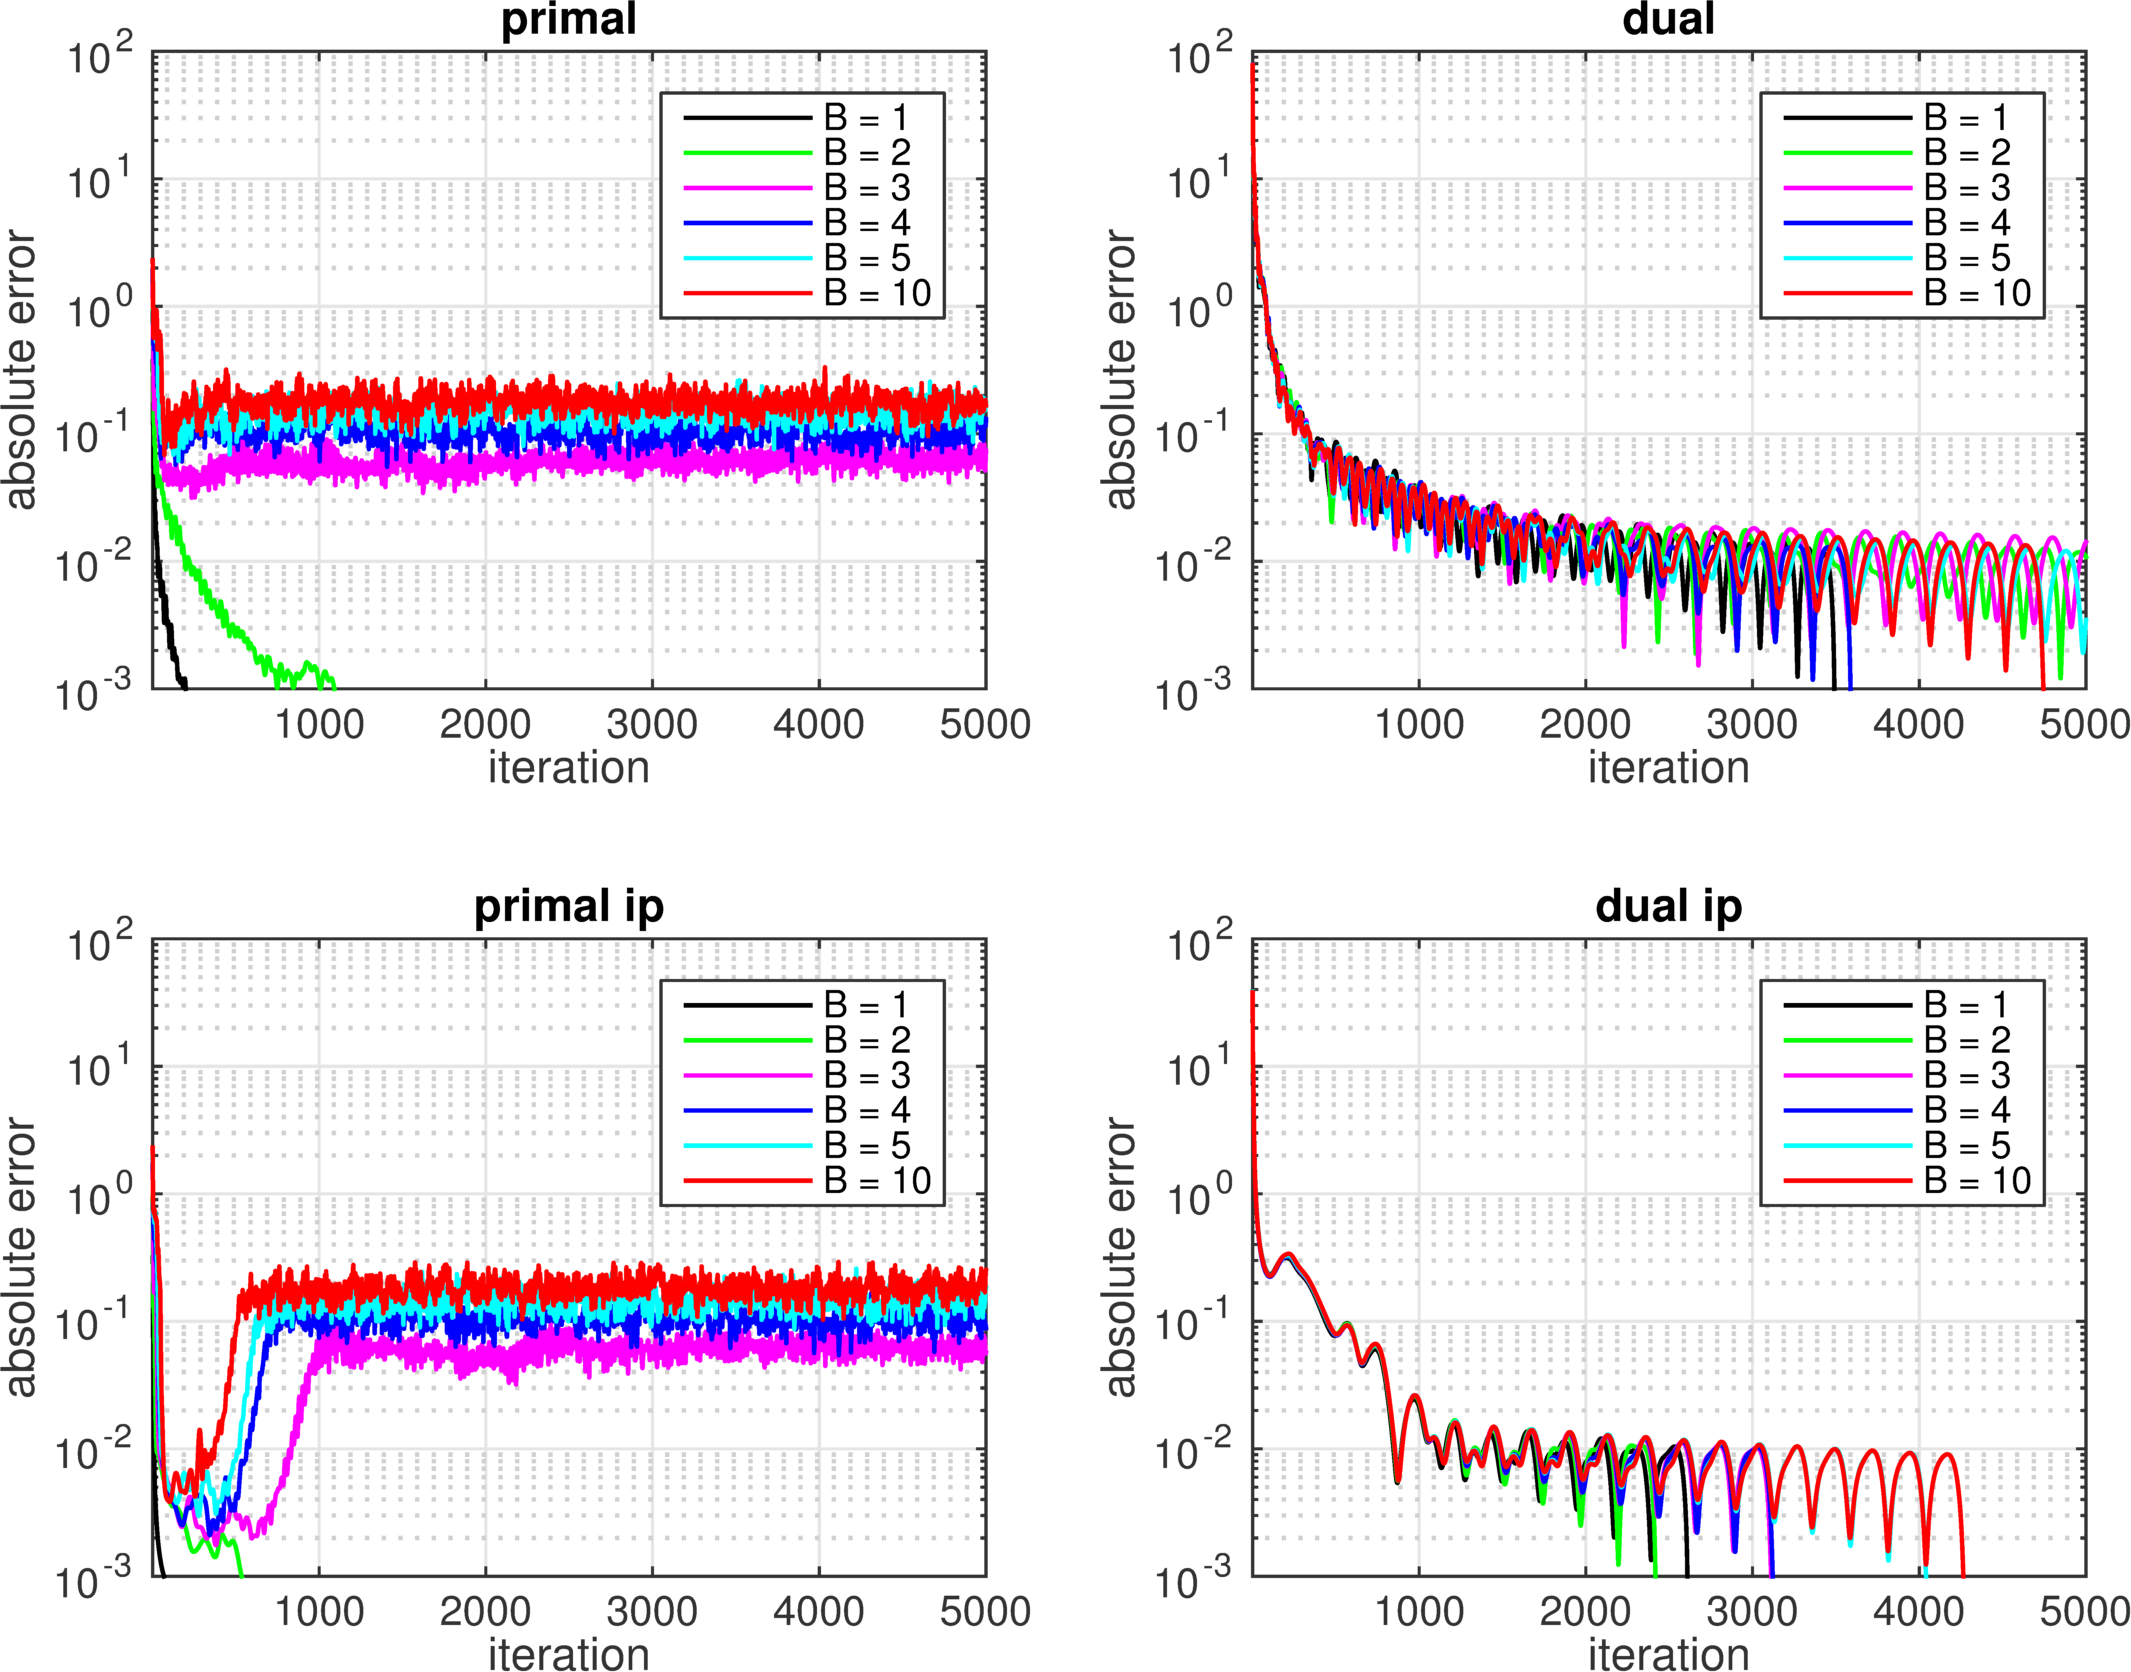
\includegraphics[width=\textwidth]{../figures/noprecond_norndperm.png}
	\caption{Results on a random LP problem of size $50 \times 300$. No preconditioning and no random permutation.}
	\label{fig:nop_nor}
\end{figure*}

\subsection*{Block-splitting with Random Permutation (No Preconditioning)}

In this set of experiments, we randomly permuted the update order of the block variables at each iteration. The results are shown in Figure \ref{fig:nop_r}. When using random permutation, the primal now converges for all block sizes. Note that splitting the primal into more blocks requires more iterations. However, performing block splitting may still result in lower overall runtime because of the faster inverse computations. 

\begin{figure*}[h]
	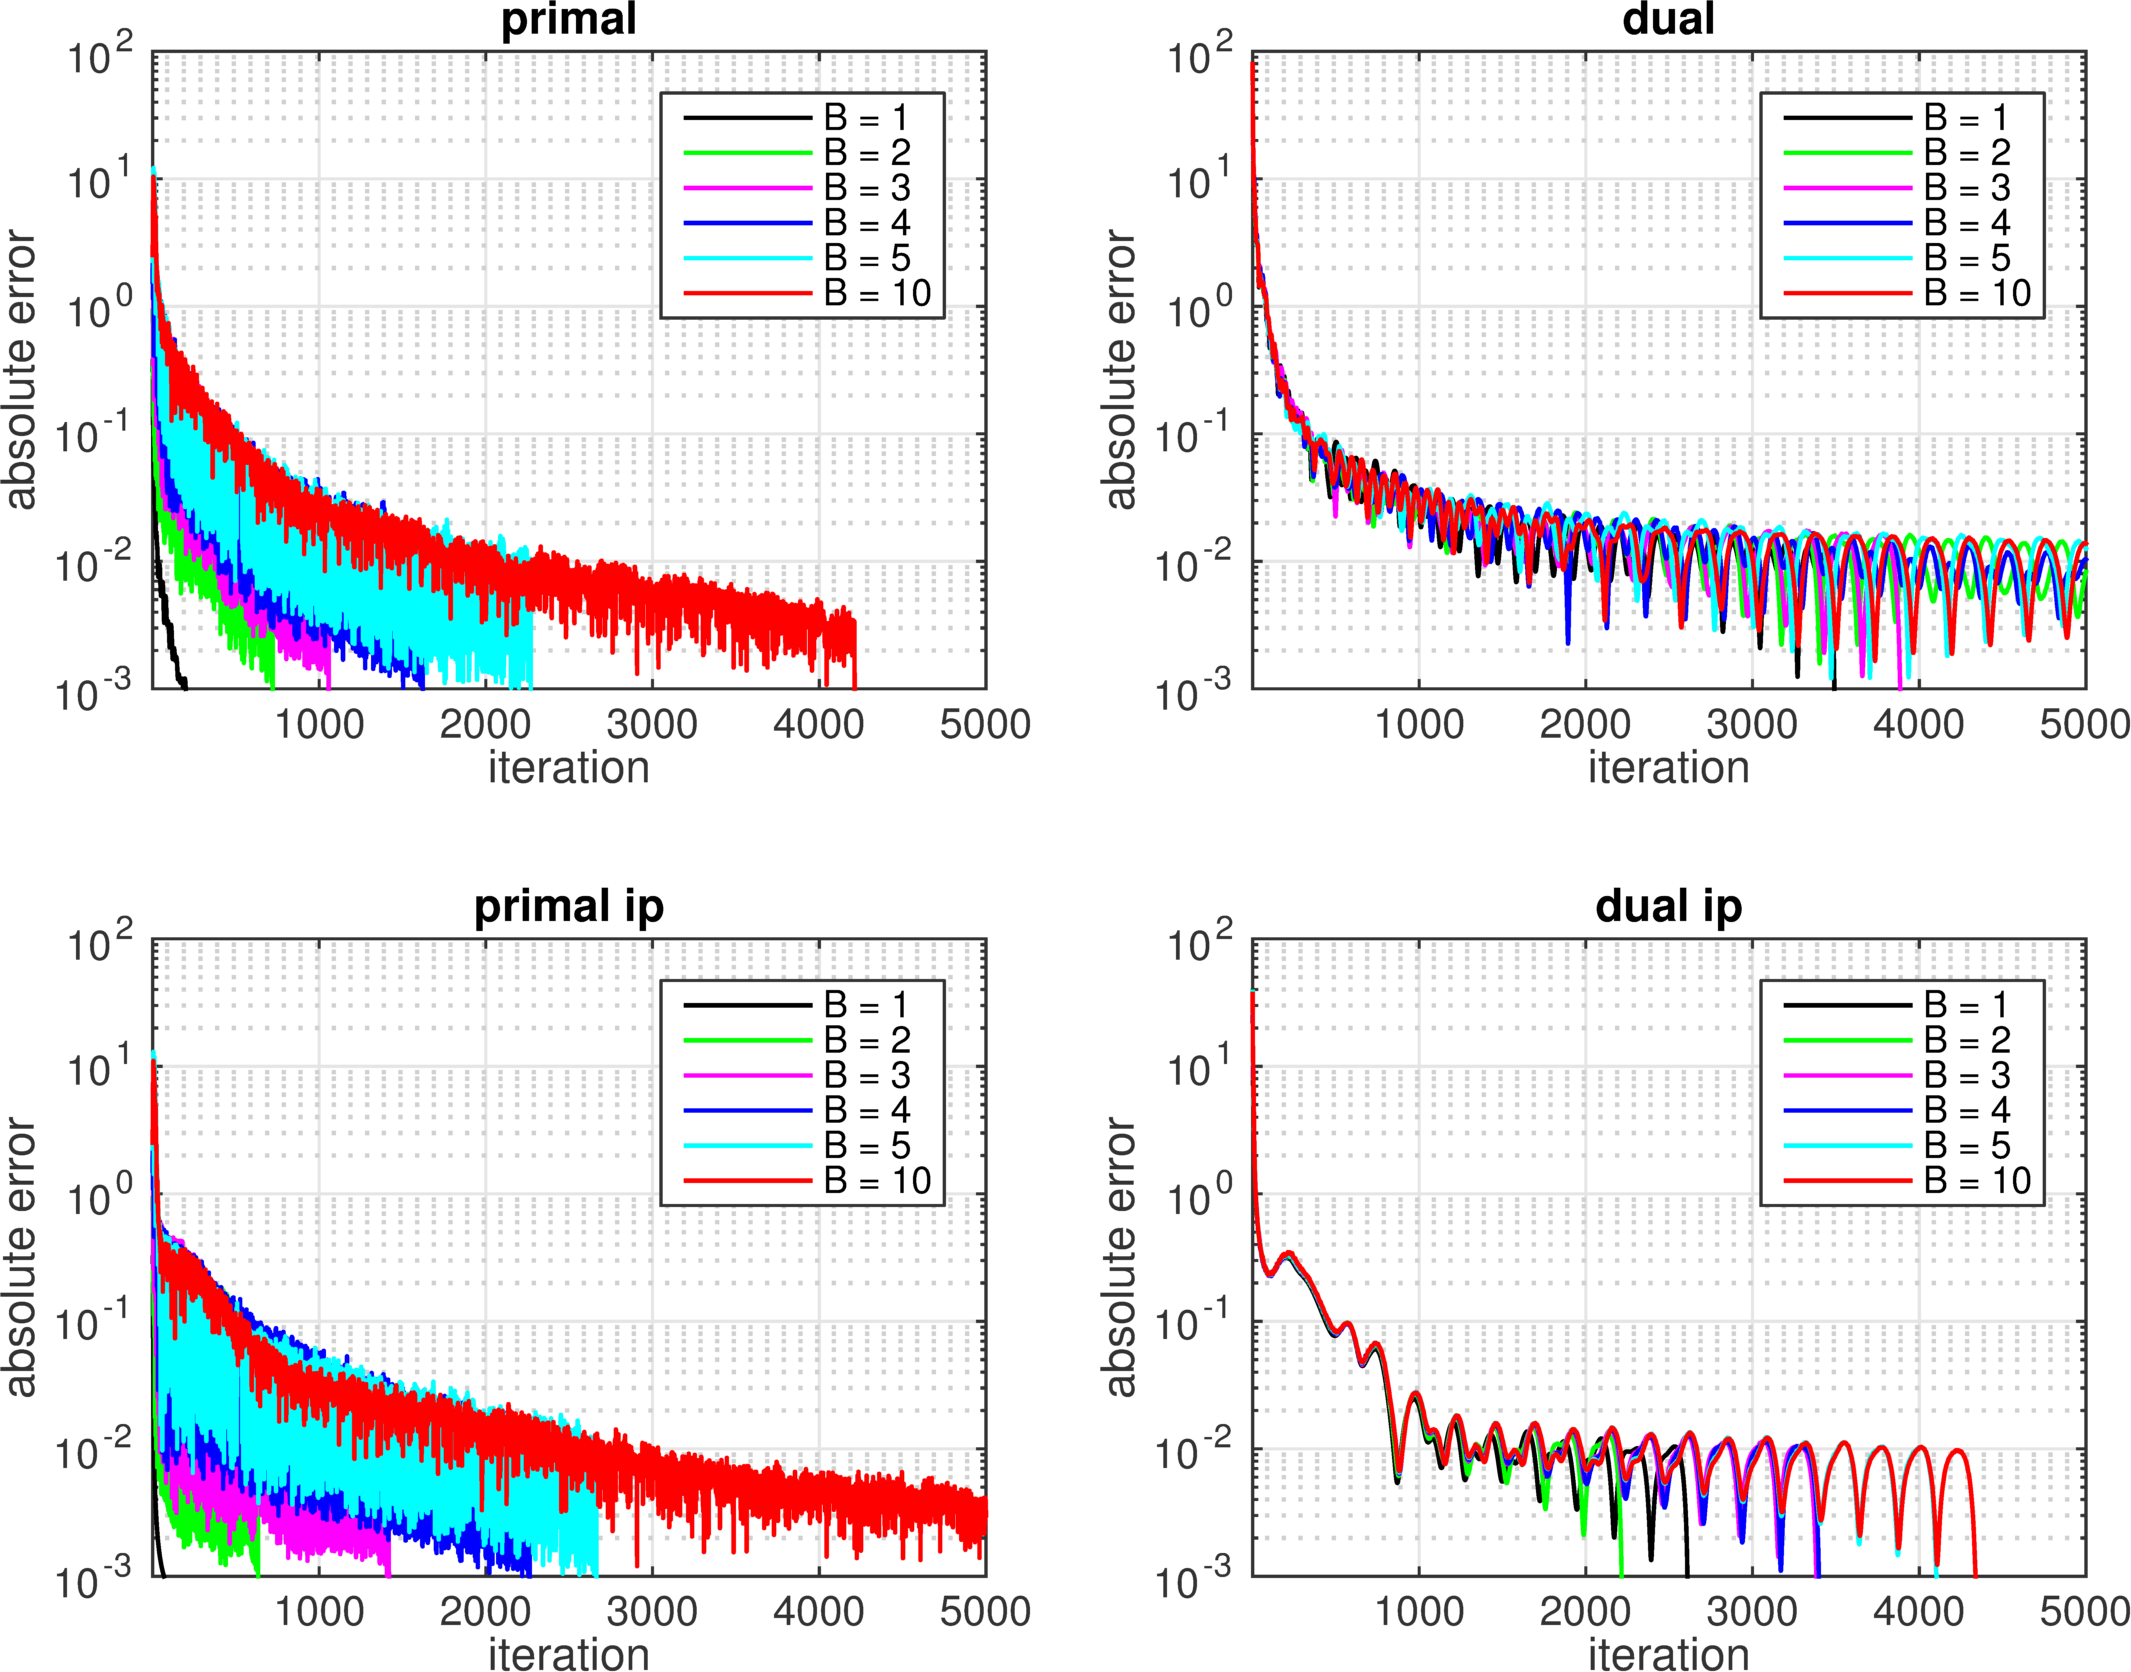
\includegraphics[width=\textwidth]{../figures/noprecond_rndperm.png}
	\caption{Results on a random LP problem of size $50 \times 300$. Only random permutation and no preconditioning.}
	\label{fig:nop_r}
\end{figure*}

\subsection*{Block-splitting with Standard Preconditioning (No Random Permutation)}
In this set of experiments, we applied standard preconditioning to each problem and used sequential block updates (no random permutation). The results are shown in Figure \ref{fig:p_nor}. Note that the number of blocks has no effect on the number of iterations required for either dual algorithm. We explain this behavior in the appendix. 

These results suggest that one should prefer to use the maximum number of blocks possible ($n$ for the primal and $m$ for the dual) when using preconditioning. In this case, the matrices that need to be inverted in the decision variable updates become scalars, so the updates can be computed rapidly.

\begin{figure*}[h]
	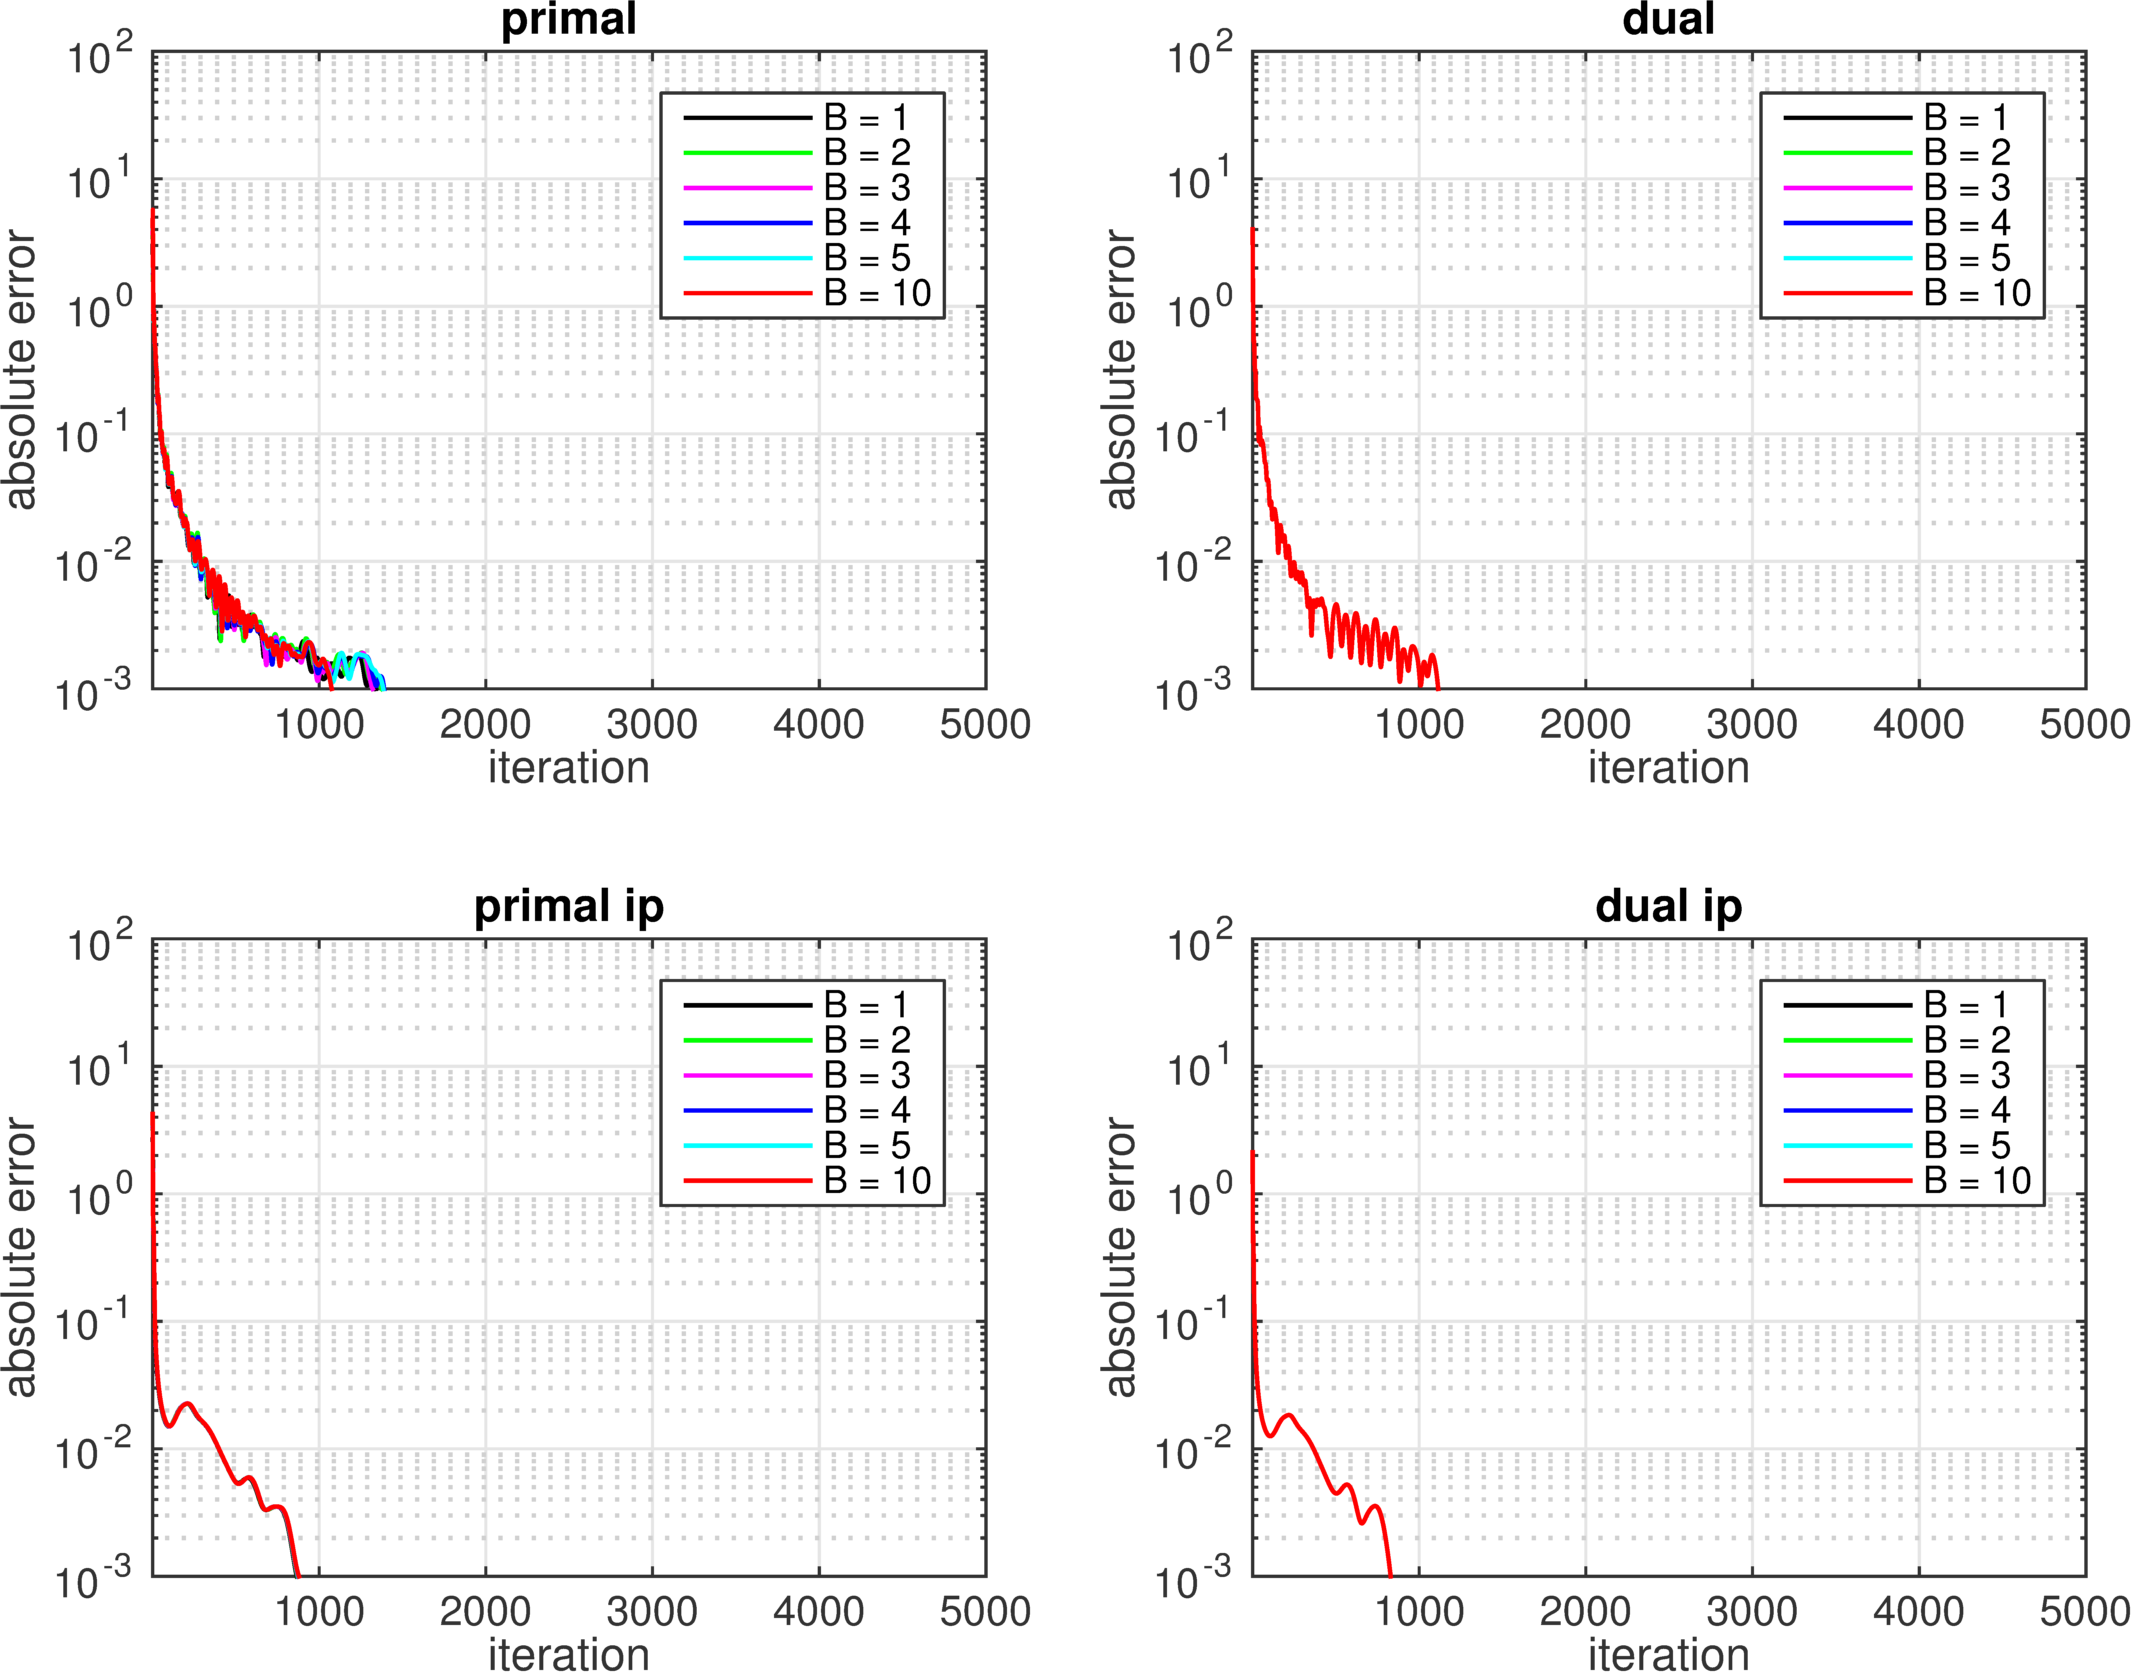
\includegraphics[width=\textwidth]{../figures/precond_norndperm.png}
	\caption{Results on a random LP problem of size $50 \times 300$. Only preconditioning and no random permutation.}
	\label{fig:p_nor}
\end{figure*}

\subsection*{Preconditioning with no Block-Splitting}

We also studied the effect of preconditioning (without block-splitting) on the convergence rate of the basic primal and dual ADMM algorithms applied to \eqref{eq:LPR} and \eqref{eq:LDR}. We generated 10 random problems of size $50 \times 300$ and recorded the number of iterations required to converge as a function of $\beta$. The results  are shown in Figure \ref{fig:base_p_d}. We observe that all of the ADMM approaches are relatively insensitive to $\beta$.

\begin{figure*}[ht]
	\centering
	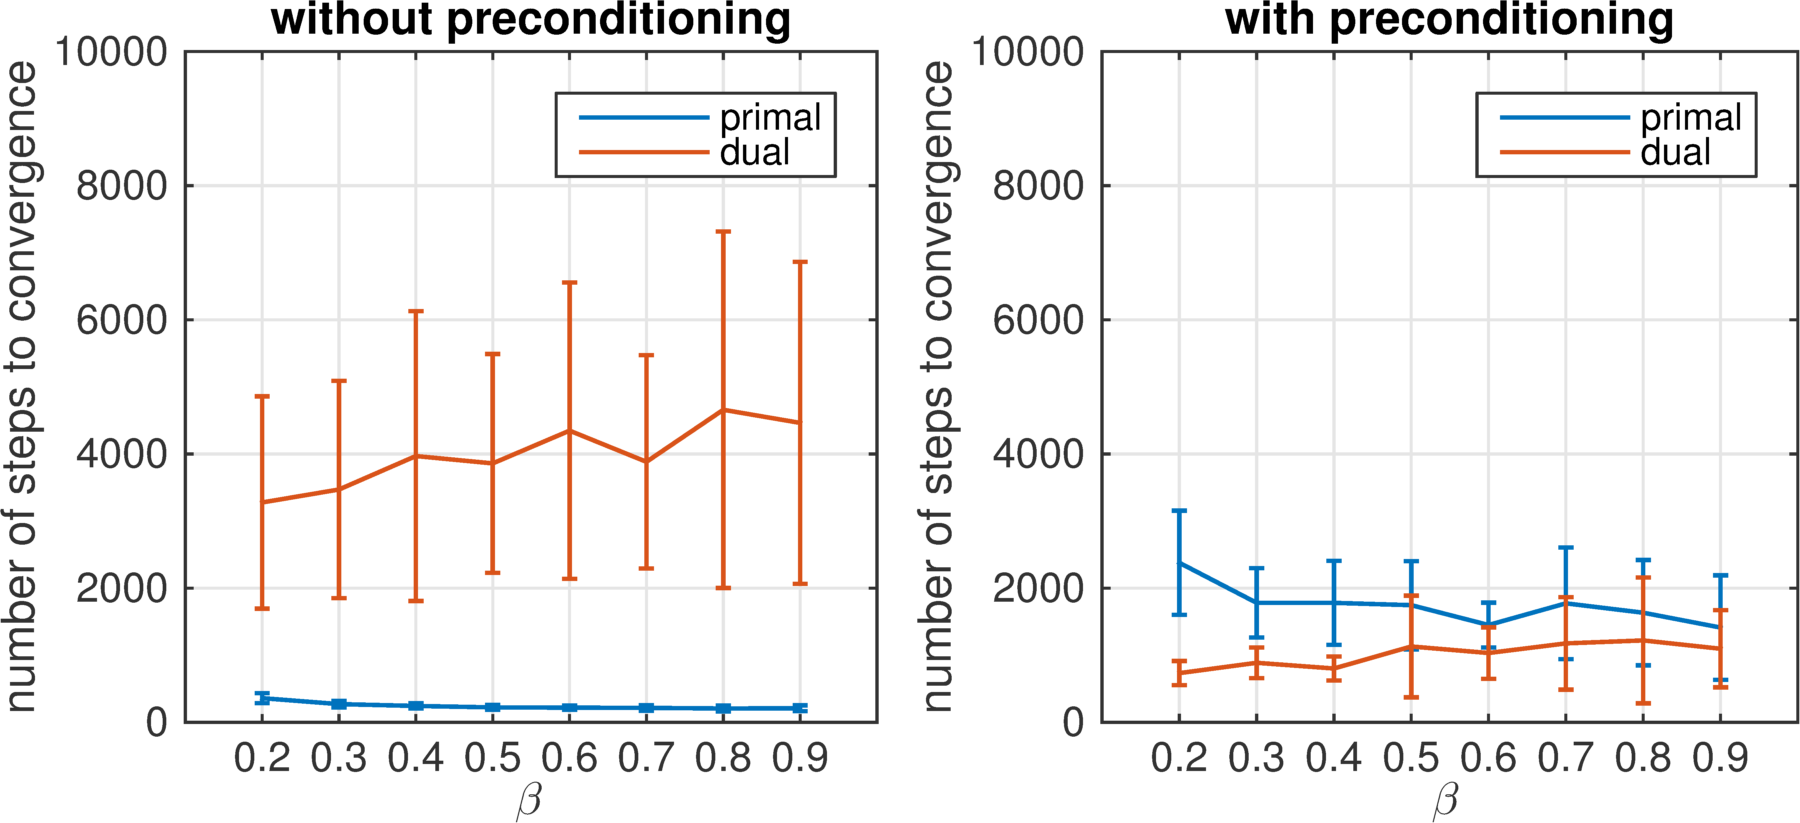
\includegraphics[width=0.8\textwidth]{../figures/primal_dual_preconditioning.png}
	\caption{Results on 10 random LP problem of size $50 \times 300$ using standard preconditioning. }
	\label{fig:base_p_d}
\end{figure*}

\subsection*{Cholesky and Incomplete Cholesky Preconditioning}
We then generated a random problem of size $100\times500$ and recorded the number of iterations required for various preconditioning approaches to converge. Figures \ref{fig:ichol_primal} and \ref{fig:ichol_dual} show the results of this experiment applied to \eqref{eq:LPR} and \eqref{eq:LDR}, respectively. We observe that Cholesky and incomplete Cholesky preconditioning have essentially the same convergence behavior as standard preconditioning (as long as the incomplete Cholesky drop tolerance is not set too high).

We then tested the speed of the different preconditioning techniques. Figure \ref{fig:ichol_primal_speed} shows that the Cholesky preconditioning step is faster than that of standard preconditioning, but the incomplete Cholesky preconditioning step is even faster. However, in our experiments, nearly all of the computation time was spent inside the solvers. This may be due to the implementation of the solvers, which we intend to improve in our future work.

\begin{figure*}[ht]
	\centering
	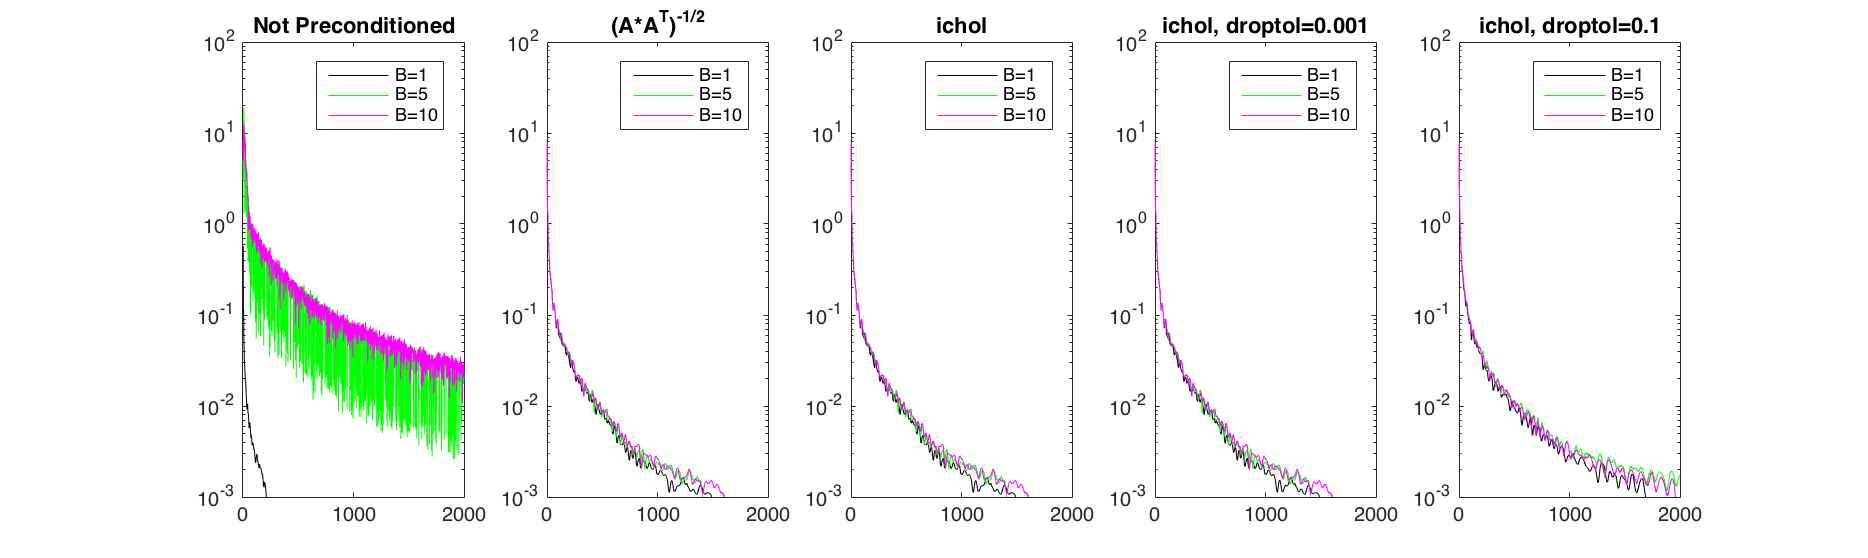
\includegraphics[width=1.0\textwidth]{../../experiments/incomplete_cholesky/ichol_droptol_conv_primal.png}
	\caption{Comparison of preconditioning techniques for primal: not preconditioned, standard preconditioning, cholesky, and incomplete cholesky using 2 different drop tolerances. Size of $A$: $100 \times 500$.}
	\label{fig:ichol_primal}
\end{figure*}

\begin{figure*}[ht]
	\centering
	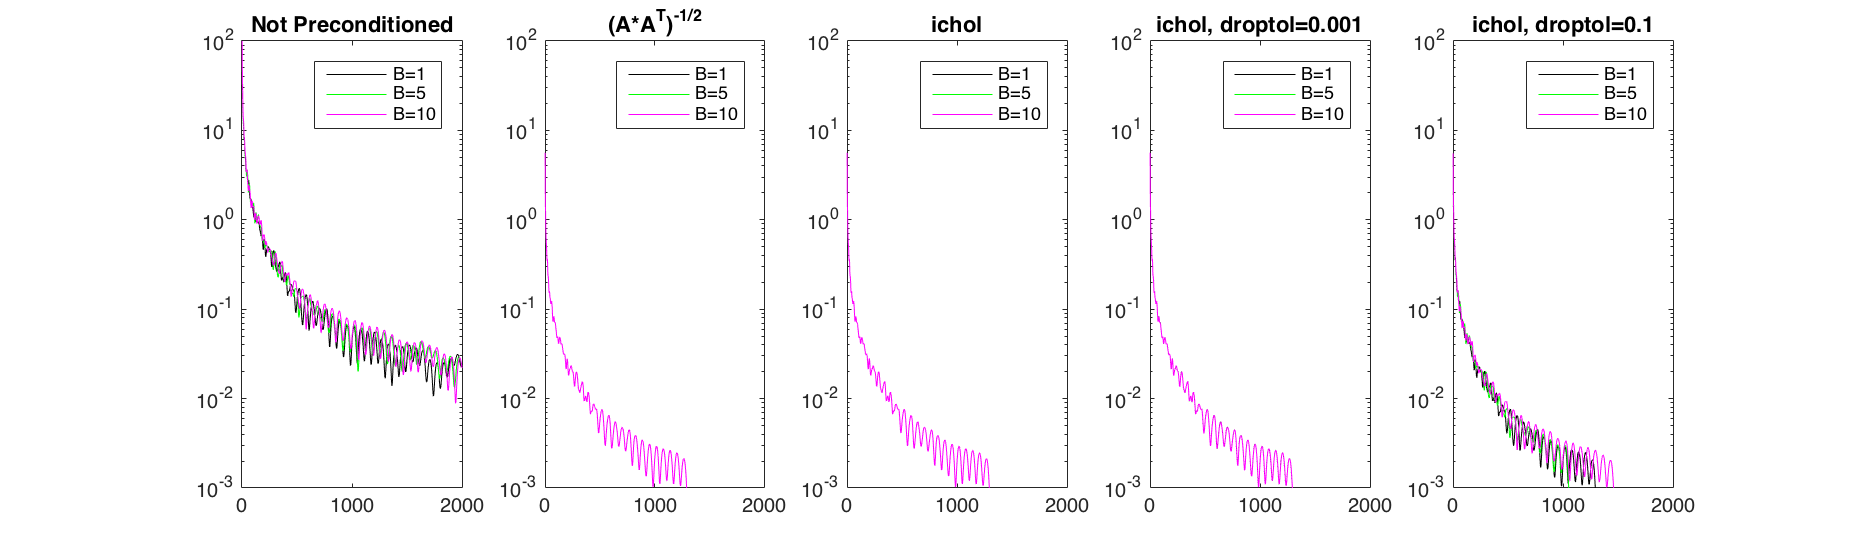
\includegraphics[width=1.0\textwidth]{../../experiments/incomplete_cholesky/ichol_droptol_conv_dual.png}
	\caption{Comparison of preconditioning techniques for dual: not preconditioned, standard preconditioning, cholesky, and incomplete cholesky using 2 different drop tolerances. Size of $A$: $100 \times 500$.}
	\label{fig:ichol_dual}
\end{figure*}

\begin{figure*}[ht]
	\centering
	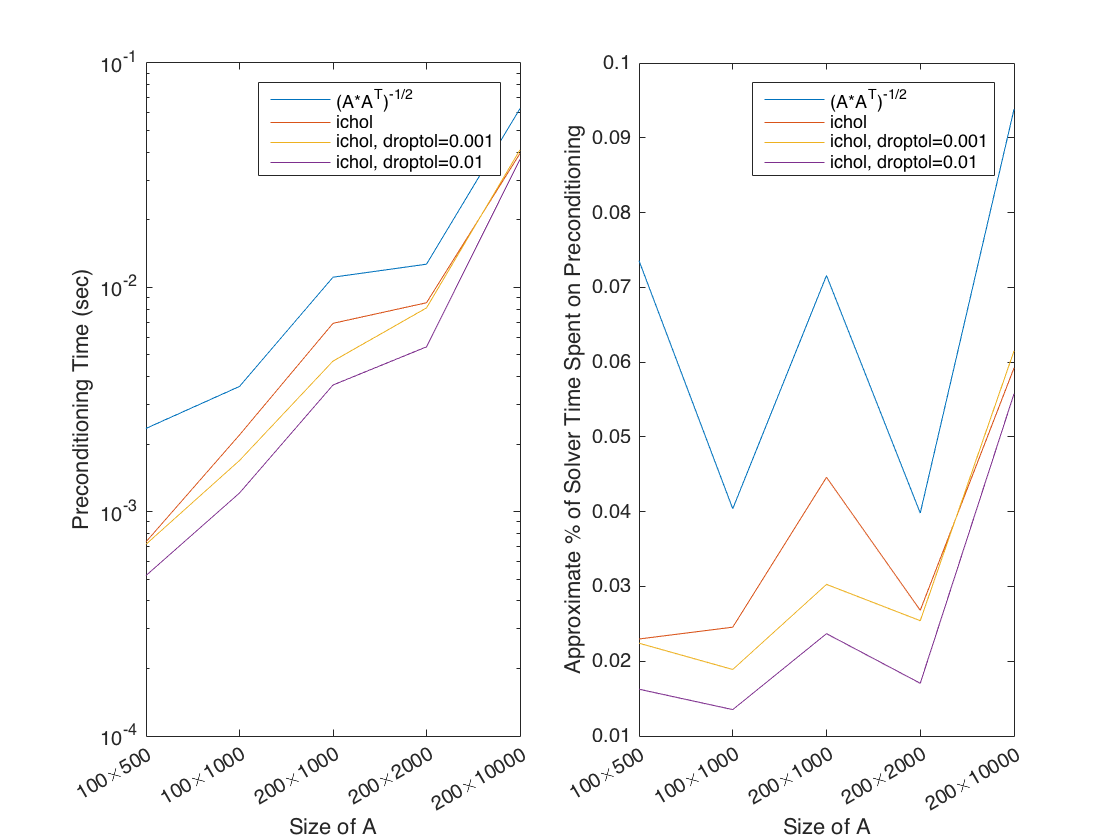
\includegraphics[height=0.5\textwidth]{../../experiments/incomplete_cholesky/ichol_speed_primal_various_A.png}
	\caption{Preconditioning speed for primal LP. Left figure: Time required to perform preconditioning step. Right figure: Percentage of overall solver time spent on the preconditioning step.}
	\label{fig:ichol_primal_speed}
\end{figure*}

\subsection*{SDP}

Finally, we randomly generated a problem of size $m=30$, $n=10$ and recorded the number of steps required for the SDP primal and SDP dual solvers to converge for various values of $\beta$. The results are shown in Figures \ref{fig:sdp_primal} and \ref{fig:sdp_dual}. The dashed lines correspond to $\beta$ values selected using the following rules:
\begin{eqnarray*}
\text{Primal:} & \beta=\text{trace}(A^{T}A)/n^{2}\\
\text{Dual:} & \beta=\text{trace}(AA^{T})/n
\end{eqnarray*}

\begin{figure*}[ht]
	\centering
	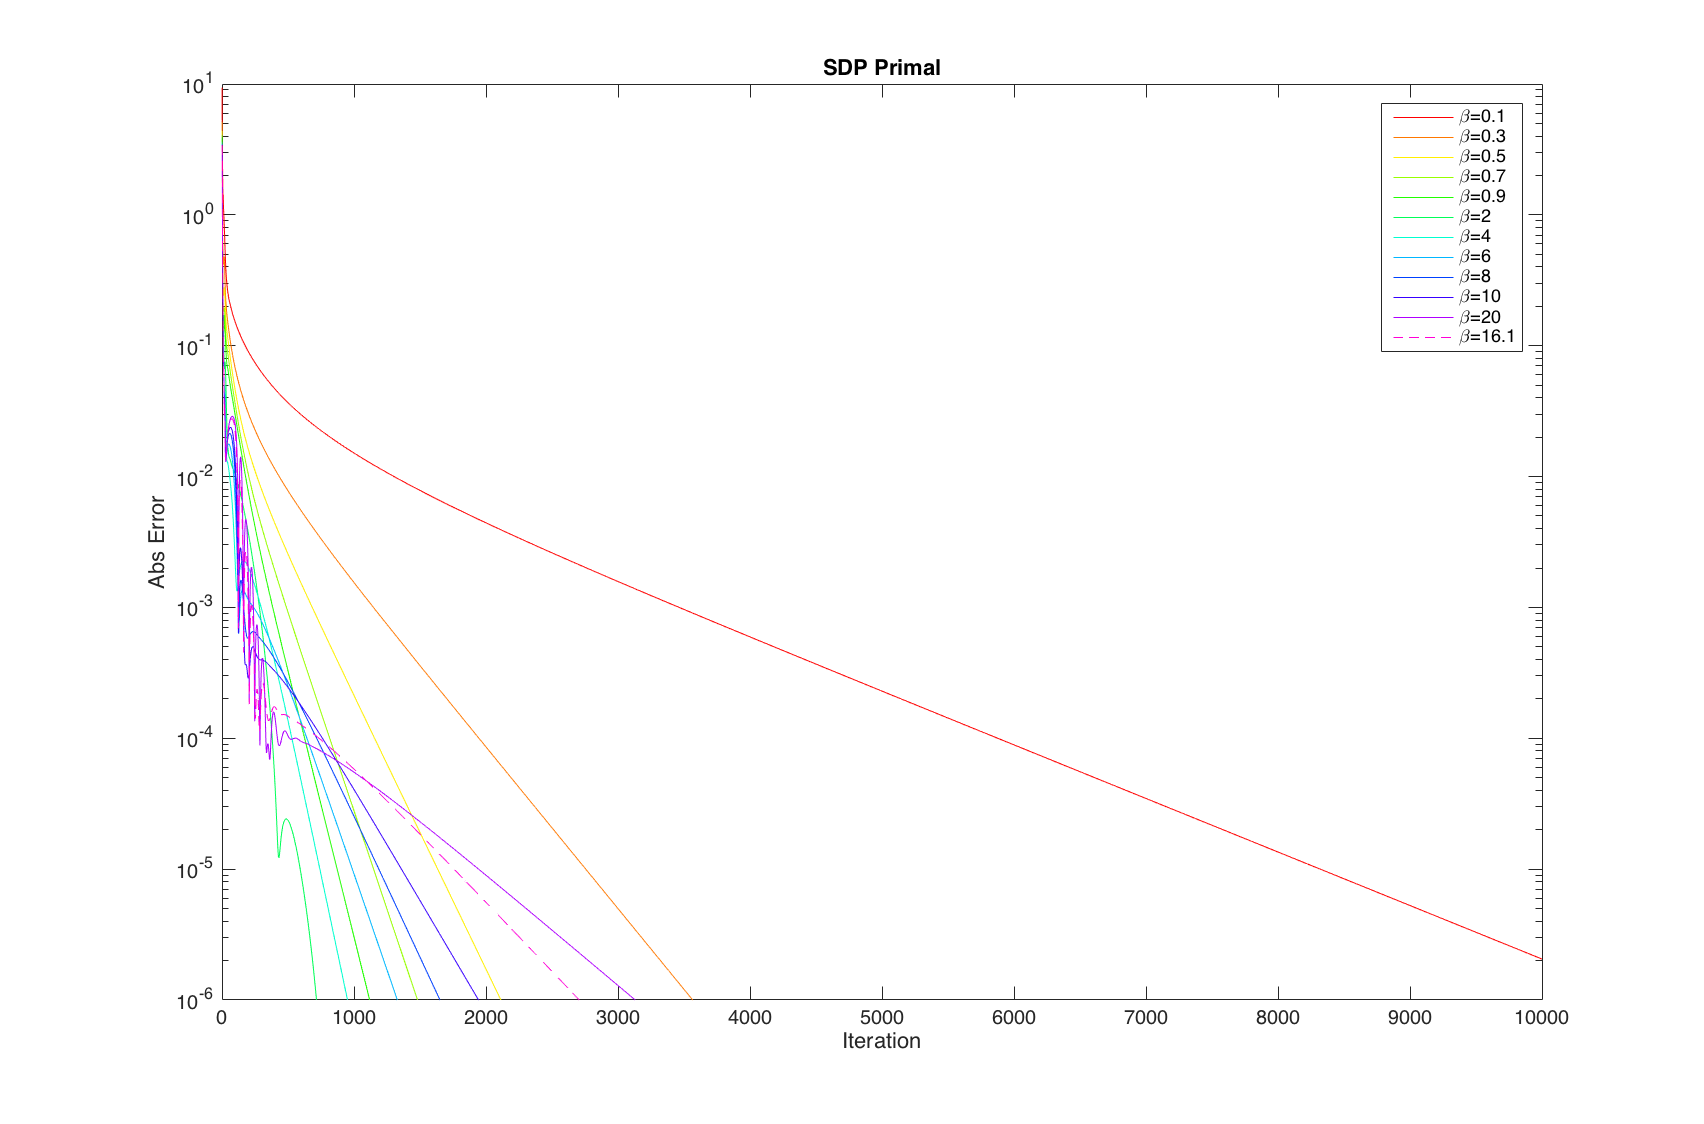
\includegraphics[width=0.8\textwidth]{/Users/nicochaves/Documents/Stanford/MSE310_Project/admm-for-lp/experiments/sdp/results/sdp_primal_results_m_30_n_10}
	\caption{SDP Primal, $m=30, n=10$}
	\label{fig:sdp_primal}
\end{figure*}

\begin{figure*}[ht]
	\centering
	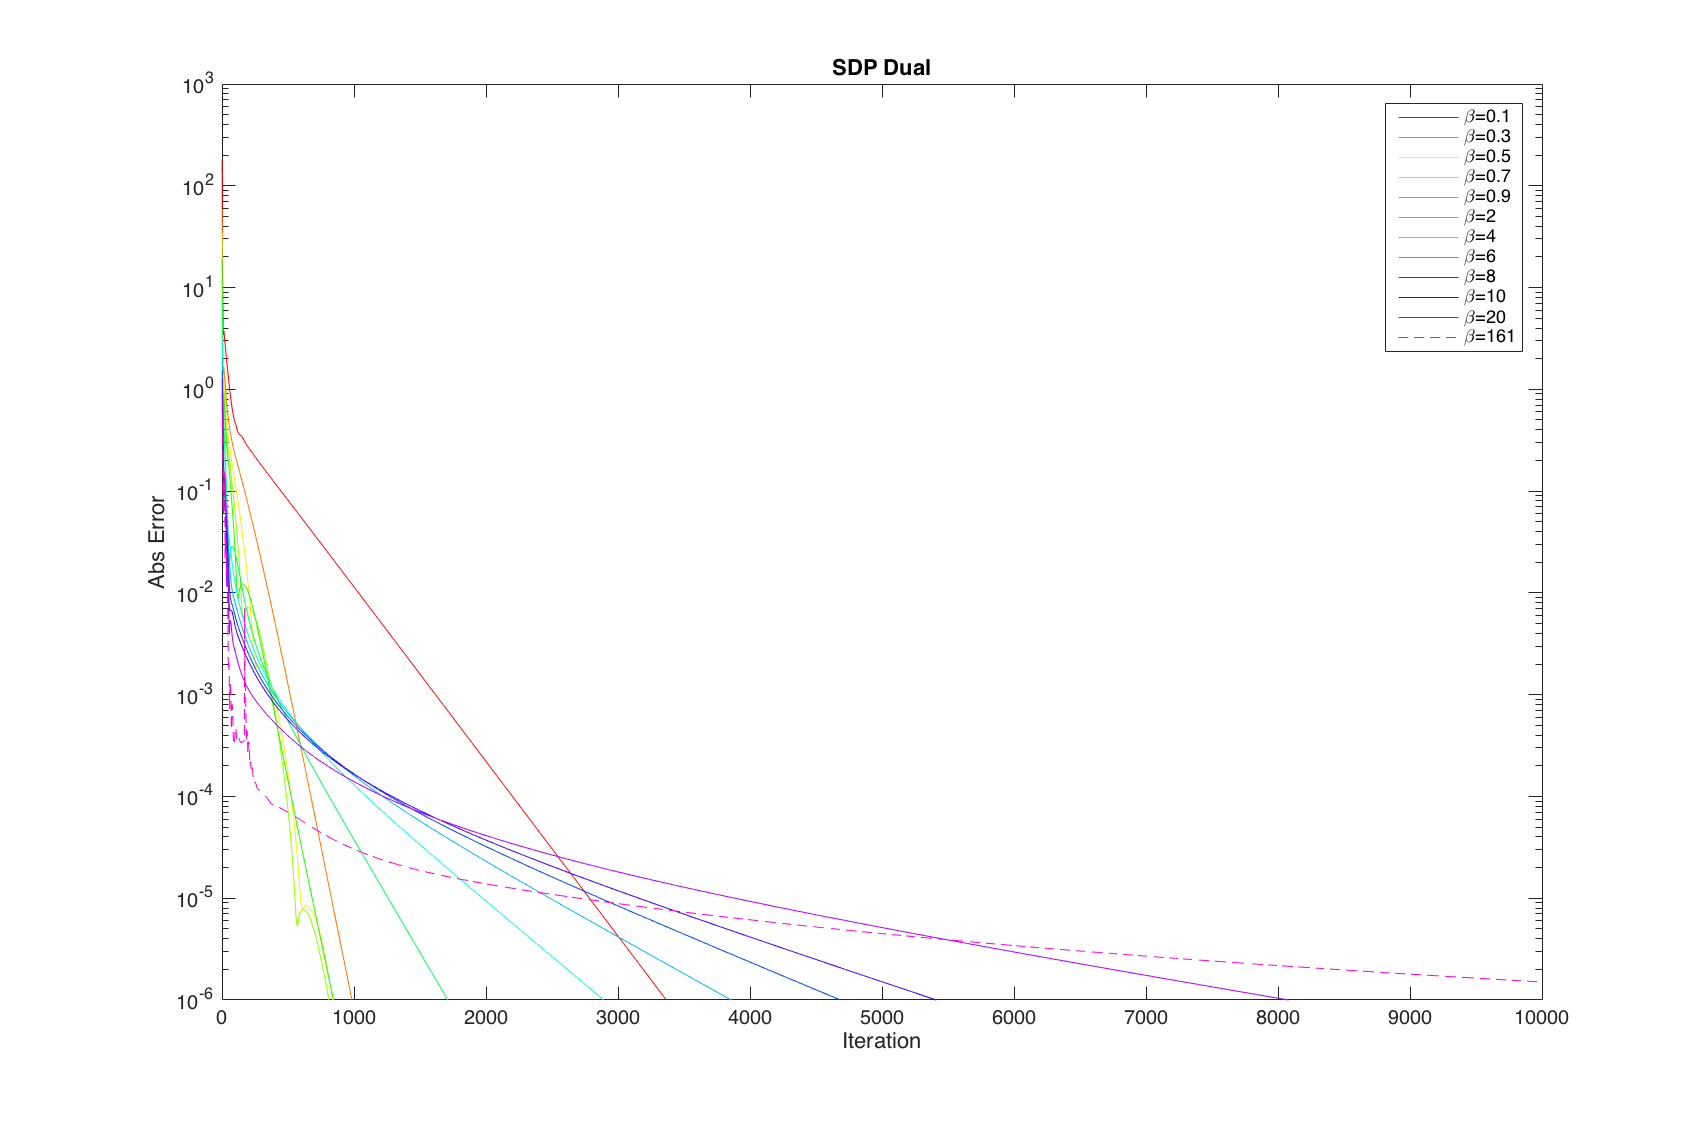
\includegraphics[width=0.8\textwidth]{/Users/nicochaves/Documents/Stanford/MSE310_Project/admm-for-lp/experiments/sdp/results/sdp_dual_results_m_30_n_10}
	\caption{SDP Dual, ,$m=30, n=10$}
	\label{fig:sdp_dual}
\end{figure*}

We observe that the solvers are somewhat sensitive to $\beta$, especially for very small and very large values. 

\textbf{Note:} For the dual SDP, we tried updating $y$ and $S$ in different orders (i.e. $y$ first then $S$ and vice versa), but the differences with the above figure were negligible. This suggests that the $y$ and $S$ update order is not necessarily important.


\vspace{0.1in}
\section{Conclusions and Future Work}

We evaluated the performance of several variants of ADMM for linear and semidefinite programs. Our experiments show that one can split linear programs into blocks without significantly increasing the number of iterations required to find an optimal solution. However, one must be sure to apply preconditioning to the problem and/or use a randomly permuted update order. 

In the future, we intend to run more experiments with the SDP solvers and try to find a robust rule to select $\beta$. We also plan to improve the speed of our LP solver implementations. If the solvers ran faster, then preconditioning could lead to more significant performance benefits.

\section{Acknowledgements}

We'd like to thank Professor Yinyu Ye for his mentorship and guidance throughout the project. 

\section{Appendix}

\subsection*{LP Primal Update Derivation}
To solve \eqref{eq:LPR}, we update $\mathbf{x}_{1}$ and $\mathbf{x}_{2}$ sequentially using:
\begin{align}
\mathbf{x}_{1}^{k+1} & = \arg \min_{\mathbf{x}_{1}^{k}} L^{P}(\mathbf{x}_{1}^{k},\mathbf{x}_{2}^{k},\mathbf{y}^{k},\mathbf{s}^k),\\
\mathbf{x}_{2}^{k+1} & = \arg \min_{\mathbf{x}_{2}^{k} \geq 0} L^{P}(\mathbf{x}_{1}^{k+1},\mathbf{x}_{2}^{k},\mathbf{y}^{k},\mathbf{s}^k).
\end{align}
Using the 1st order gradient condition
\[
\nabla_{\mathbf{x}_{1}}L^{P}(\mathbf{x}_{1},\mathbf{x}_{2},\mathbf{y}, \mathbf{s})=\mathbf{c}-A^{T}\mathbf{y}-\mathbf{s}+\beta\left(A^{T}\left(A\mathbf{x}_{1}-\mathbf{b}\right)+\left(\mathbf{x}_{1}-\mathbf{x}_{2}\right)\right) = \mathbf{0}
\]
we obtain the update step for $\mathbf{x}_{1}$
\begin{align}\label{eq:x1_primal_update_app}
\mathbf{x}_{1}^{k+1} = \left(A^{T}A+I\right)^{-1}\left(\frac{1}{\beta}A^{T}\mathbf{y}^k+\frac{1}{\beta}\mathbf{s}^k-\frac{1}{\beta}\mathbf{c}+A^{T}\mathbf{b}^k+\mathbf{x}_{2}^k\right)
\end{align}
Similarly, we solve
\[
\nabla_{\mathbf{x}_{2}}L^{P}(\mathbf{x}_{1},\mathbf{x}_{2},\mathbf{y}, \mathbf{s})=\mathbf{s}+\beta\left(\mathbf{x}_{2}-\mathbf{x}_{1}\right) = \mathbf{0}
\]
to obtain the update for $\mathbf{x}_{2}$. Since the elements of $\mathbf{x}_{2}$ are separable, we can update each one independently as follows:
\begin{align}
{x}_{2,j}^{k+1} = \max\left\{ {x}_{1,j}^{k+1}-\frac{1}{\beta}{s}_j^k,0\right\} \text{ for $j = 1,..,n$}.
\end{align}
Next, we update the multipliers $\mathbf{y}$ and $\mathbf{s}$ using steepest ascent:
\begin{align}\label{eq:y_primal_update_app}
\mathbf{y}^{k+1} &= \mathbf{y}^{k} + \beta (A \mathbf{x}_1^{k+1}  - \mathbf{b}) 
\end{align}
\begin{align}\label{eq:s_primal_update_app}
\mathbf{s}^{k+1} &= \mathbf{s}^{k}  - \beta  (\mathbf{x}_1^{k+1}  -\mathbf{x}_2^{k+1} )
\end{align}


%%%%%%%%%%
\subsection*{LP Dual Update Derivation}
To solve \eqref{eq:LDR}, we update $\mathbf{y}$ and $\mathbf{s}$ sequentially using:
\begin{align}
\mathbf{y}^{k+1} & = \arg \min_{\mathbf{y}} L^{d}(\mathbf{y}^{k},\mathbf{s}^k, \mathbf{x}^{k}),\\
\mathbf{s}^{k+1} & = \arg \min_{\mathbf{s} \geq 0} L^{d}(\mathbf{y}^{k+1},\mathbf{s}^k,\mathbf{x}^{k}).
\end{align}
Using the 1st order gradient conditions
\begin{align}
\nabla_{\mathbf{y}}L^{d}(\mathbf{y},\mathbf{s},\mathbf{x}) & =  -\mathbf{b}-A\mathbf{x}+\beta A\left(A^{T}\mathbf{y}+\mathbf{s}-\mathbf{c}\right)  = \mathbf{0}, \label{eq:dual_y_app} \\
\nabla_{\mathbf{s}}L^{d}(\mathbf{y},\mathbf{s},\mathbf{x}) & =  -\mathbf{x}+\beta\left(A^{T}\mathbf{y}+\mathbf{s}-\mathbf{c}\right) =  \mathbf{0},
\end{align}
we have the updates for $\mathbf{y}$ and $\mathbf{s}$:
\begin{align}\label{eq:y_dual_update_app}
\mathbf{y}^{k+1} = \left(AA^{T}\right)^{-1}\left(\frac{1}{\beta}\left(A\mathbf{x}^{k}+\mathbf{b}\right)-A\mathbf{s}^{k}+A\mathbf{c}\right),
\end{align}
\begin{align}\label{eq:s_dual_update_app}
s_j^{k+1} = \max\left\{ \frac{1}{\beta}{x}_j^k-(A^{T}\mathbf{y}^{k+1})_j+{c}_j,0\right\}  \text{ for $j = 1,..,n$}.
\end{align}

\subsection*{Primal ADMM with Block Splitting Derivation (B=2 Blocks)}
Here, we derive the update for the primal ADMM with block splitting. To help make our derivations concrete, we first consider splitting the problem into $B=2$ blocks of equal size as follows:
\[
\mathbf{x}_{1}=\begin{bmatrix}\mathbf{x}_{1,1}\\
\mathbf{x}_{1,2}
\end{bmatrix},
 \ \  
A=\begin{bmatrix}A_{1} & A_{2}\end{bmatrix},
\ \ 
\mathbf{c}=\begin{bmatrix}\mathbf{c}_{1}\\
\mathbf{c}_{2}
\end{bmatrix}
\]
Then the Lagrangian can be expressed as:
\begin{eqnarray*}
L^{P}(\mathbf{x}_{1},\mathbf{x}_{2},\mathbf{y}) & = & \mathbf{c}_{1}^{T}\mathbf{x}_{1,1}+\mathbf{c}_{2}^{T}\mathbf{x}_{1,2}-\mathbf{y}^{T}\left(A_{1}\mathbf{x}_{1,1}+A_{2}\mathbf{x}_{1,2}-\mathbf{b}\right)-\mathbf{s}_{1}^{T}\left(\mathbf{x}_{1,1}-\mathbf{x}_{2,1}\right)-\mathbf{s}_{2}^{T}\left(\mathbf{x}_{1,2}-\mathbf{x}_{2,2}\right)\\
 &  & +\frac{\beta}{2}\left(\left\Vert A_{1}\mathbf{x}_{1,1}+A_{2}\mathbf{x}_{1,2}-\mathbf{b}\right\Vert ^{2}+\left\Vert \mathbf{x}_{1,1}-\mathbf{x}_{2,1}\right\Vert ^{2}+\left\Vert \mathbf{x}_{1,2}-\mathbf{x}_{2,2}\right\Vert ^{2}\right)
\end{eqnarray*}
Taking the gradient with respect to the 1st block of $\mathbf{x}_{1}$:
\[
\nabla_{\mathbf{x}_{1,1}}L^{P}(\mathbf{x}_{1},\mathbf{x}_{2},\mathbf{y})=\mathbf{c}_{1}-A_{1}^{T}\mathbf{y}-\mathbf{s}_{1}+\beta\left(A_{1}^{T}\left(A_{1}\mathbf{x}_{1,1}+A_{2}\mathbf{x}_{1,2}-\mathbf{b}\right)+\left(\mathbf{x}_{1,1}-\mathbf{x}_{2,1}\right)\right)
\]
Setting the gradient to 0, we obtain the update for $\mathbf{x}_{1,1}$:
\[
\mathbf{x}_{1,1}^{k+1}=\left(A_{1}^{T}A_{1}+I\right)^{-1}\left(\frac{1}{\beta}A_{1}^{T}\mathbf{y}+\frac{1}{\beta}\mathbf{s}_{1}-\frac{1}{\beta}\mathbf{c}_{1}+A_{1}^{T}\mathbf{b}+\mathbf{x}_{2,1}^{k}-A_{1}^{T}A_{2}\mathbf{x}_{1,2}^{k}\right)
\]
By symmetry, the update step for the 2nd block of $\mathbf{x}_{1}$
is:
\[
\mathbf{x}_{1,2}^{k+1}=\left(A_{2}^{T}A_{2}+I\right)^{-1}\left(\frac{1}{\beta}A_{2}^{T}\mathbf{y}+\frac{1}{\beta}\mathbf{s}_{2}-\frac{1}{\beta}\mathbf{c}_{2}+A_{2}^{T}\mathbf{b}+\mathbf{x}_{2,2}^{k}-A_{2}^{T}A_{1}\mathbf{x}_{1,1}^{k+1}\right)
\]
Note that here we use $\mathbf{x}_{1,1}^{k+1}$ to update $\mathbf{x}_{1,2}$. Our results show that when $B>2$ blocks, one may need to randomly permute the update order. As a result, on some iterations, we may first update $\mathbf{x}_{1,2}$, then use the new value to update $\mathbf{x}_{1,1}$. One can easily extend the above derivation to a general number of blocks.  


\subsection*{Dual ADMM with Block Splitting Derivation (B=2 Blocks)}
Now, we derive the corresponding update for the dual ADMM with block splitting. Again, we first consider the $B=2$ case and split the problem into 2 blocks of equal size:

\[
\mathbf{y}=\begin{bmatrix}\mathbf{y}_{1}\\
\mathbf{y}_{2}
\end{bmatrix},
\ \
A^{T}=\begin{bmatrix}A_{1}^{T} & A_{2}^{T}\end{bmatrix},
\ \ 
\mathbf{b}=\begin{bmatrix}\mathbf{b}_{1}\\
\mathbf{b}_{2}
\end{bmatrix}
\]

Then the Lagrangian can be expressed as:

\[
L^{d}(\mathbf{y},\mathbf{s},\mathbf{x})=-\mathbf{b}_{1}^{T}\mathbf{y}_{1}-\mathbf{b}_{2}^{T}\mathbf{y}_{2}-\mathbf{x}^{T}\left(A_{1}^{T}\mathbf{y}_{1}+A_{2}^{T}\mathbf{y}_{2}+\mathbf{s}-\mathbf{c}\right)+\frac{\beta}{2}\left\Vert A_{1}^{T}\mathbf{y}_{1}+A_{2}^{T}\mathbf{y}_{2}+\mathbf{s}-\mathbf{c}\right\Vert ^{2}
\]


Differentiating with respect to $\mathbf{y}_{1}$:

\[
\nabla_{\mathbf{y}_{1}}L^{d}(\mathbf{y},\mathbf{s},\mathbf{x})=-\mathbf{b}_{1}-A_{1}\mathbf{x}+\beta A_{1}\left(A_{1}^{T}\mathbf{y}_{1}+A_{2}^{T}\mathbf{y}_{2}+\mathbf{s}-\mathbf{c}\right)
\]

Setting the gradient to 0, we obtain the update for $\mathbf{y}_{1}$:
\begin{eqnarray*}
A_{1}\left(A_{1}^{T}\mathbf{y}_{1}^{k+1}+A_{2}^{T}\mathbf{y}_{2}^{k}+\mathbf{s}-\mathbf{c}\right) & = & \frac{1}{\beta}\left(A_{1}\mathbf{x}+\mathbf{b}_{1}\right)\\
A_{1}A_{1}^{T}\mathbf{y}_{1}^{k+1} & = & \frac{1}{\beta}\left(A_{1}\mathbf{x}+\mathbf{b}_{1}\right)-A_{1}\left(A_{2}^{T}\mathbf{y}_{2}^{k}+\mathbf{s}-\mathbf{c}\right)\\
\mathbf{y}_{1}^{k+1} & = & \left(A_{1}A_{1}^{T}\right)^{-1}\left(\frac{1}{\beta}\left(A_{1}\mathbf{x}+\mathbf{b}_{1}\right)-A_{1}\left(A_{2}^{T}\mathbf{y}_{2}^{k}+\mathbf{s}-\mathbf{c}\right)\right)
\end{eqnarray*}


By symmetry, the update for $\mathbf{y}_{2}$ is:

\[
\mathbf{y}_{2}^{k+1}=\left(A_{2}A_{2}^{T}\right)^{-1}\left(\frac{1}{\beta}\left(A_{2}\mathbf{x}+\mathbf{b}_{2}\right)-A_{2}\left(A_{1}^{T}\mathbf{y}_{1}^{k+1}+\mathbf{s}-\mathbf{c}\right)\right)
\]


assuming that we update $\mathbf{y}_{2}$ after $\mathbf{y}_{1}$. As in the primal case, we may need to randomly permute the update order at each iteration. One can easily extend the above derivation to a general number of blocks. 


{ \subsection*{Using Preconditioning for Dual Block Splitting}
When preconditioning is applied to the dual LP problem (whether or not implemented with the interior point method), the variables $\mathbf{y}$ become separable. To see this, consider \eqref{eq:dual_y_app}, where the coefficient of $\mathbf{y}$ is $A A^T$. When standard preconditioning is applied, we have
\[
A' (A')^T  = (AA^T )^{-1/2}A A^T (AA^T )^{-1/2} =  (AA^T )^{-1/2}(AA^T )^{1/2} (AA^T )^{1/2} (AA^T )^{-1/2}  = I.
\]
Therefore, the variables in $\mathbf{y}$ become separable and block-splitting produces the same result as non-block-splitting. This explains the dual experiments, where the number of iterations required by the dual is independent of the number of blocks when preconditioning is applied.


\subsection*{Derivation of Updates for ADMM SDP Primal}
1st order gradient condition for $X_{1}$:
\[
\nabla_{X_{1}}L=C-\mathcal{A}^{T}y-Z+\beta\mathcal{A}^{T}\left(\mathcal{A}X_{1}-b\right)+\beta\left(X_{1}-X_{2}\right)=\mathbf{0}
\]
where 
\[
\mathcal{A}^{T}y=\sum_{i=1}^{m}y_{i}A_{i}
\]
$X_{1}$ update:
\[
X_{1}=\left(\mathcal{A}^{T}\mathcal{A}+I\right)^{-1}\left(X_{2}+\frac{1}{\beta}\left(\mathcal{A}^{T}y+Z-C\right)+\mathcal{A}^{T}b\right)
\]
1st order condition for $X_{2}$:
\[
\nabla_{X_{2}}L=-Z-\beta\left(X_{1}-X_{2}\right)=\mathbf{0}
\]
The $X_{2}$ update uses this 1st order condition and enforces the PSD requirement:
\[
X_{2} = \max\{0,-\frac{Z}{\beta}-X_{1}\}
\]
The operation $\max\{0,M\}$ was defined previously.

\subsection*{Derivation of Updates for ADMM SDP Dual}
The 1st order gradient condition for \textbf{$y$}
\[
\nabla_{y}L=\mathbf{b}-\mathcal{A}X+\beta\mathcal{A}\left(\mathcal{A}^{T}\mathbf{y}+S-C\right)=\mathbf{0}
\]
leads to the $y$ update:
\[
y=\left(\mathcal{A}\mathcal{A}^{T}\right)^{-1}\left(\frac{1}{\beta}\left(\mathcal{A}X-b\right)+\mathcal{A}\left(C-S\right)\right)
\]
The 1st order condition for \textbf{$S$}
\[
\nabla_{S}L=-X+\beta\left(\mathcal{A}^{T}\mathbf{y}+S-C\right)=\mathbf{0}
\]
leads to the $S$ update (which must enforce the PSD constraint):
\[
S=\max\left\{ 0,\frac{1}{\beta}X+C-\mathcal{A}^{T}y\right\} 
\]
Again, the operation $\max\{0,M\}$ was defined previously.

\newpage
\vspace{0.4in}
%\bibliographystyle{plain}
\bibliographystyle{ieeetr}
\end{document}
